\section{逻辑回归之多分类（数字识别）}
\label{sec:chapter6}

\subsection{数据读入与显示}

数据采用 \texttt{.mat} 格式，可以使用 \texttt{scipy} 中的 \texttt{loadmat} 方法读取：

\begin{lstlisting}[language=Python]
import numpy as np
from scipy.io import loadmat

data = loadmat('ex3data1.mat')
print(data)
print(data['X'].shape)
print(data['y'].shape)
```

```
{'__header__': b'MATLAB 5.0 MAT-file, Platform: GLNXA64, Created on: Sun Oct 16 13:09:09 2011', '__version__': '1.0', '__globals__': [], 'X': array([[0., 0., 0., ..., 0., 0., 0.],
       [0., 0., 0., ..., 0., 0., 0.],
       [0., 0., 0., ..., 0., 0., 0.],
       ...,
       [0., 0., 0., ..., 0., 0., 0.],
       [0., 0., 0., ..., 0., 0., 0.],
       [0., 0., 0., ..., 0., 0., 0.]]), 'y': array([[10],
       [10],
       [10],
       ...,
       [ 9],
       [ 9],
       [ 9]], dtype=uint8)}
(5000, 400)
(5000, 1)
\end{lstlisting}

文件中共有 $5000$ 个样本。每个样本的输入是由 $20\times 20$ 灰度图像展开得到的 $400$ 维向量，输出为图像对应的数字标签。

\begin{note}
由于 \texttt{MATLAB} 或 \texttt{Octave} 的数据约定，数字 $0$ 被标记为 $10$，使用 \texttt{Python} 时可以将其恢复为 $0$. 此外，图像数据按列展开，还原为 $20\times20$ 矩阵后需要转置。
\end{note}

\begin{lstlisting}[language=Python]
data = loadmat('ex3data1.mat')
X = data['X']
X = np.transpose(X.reshape((5000, 20, 20)), [0, 2, 1]).reshape(5000, 400)
y = data['y']
y[y==10] = 0
\end{lstlisting}

随机选取 $100$ 幅图像，显示结果如下：

\begin{lstlisting}[language=Python]
def show_a_number(num, ax):
	"""
	num.shape: (400, )
	"""
	ax.matshow(num.reshape((20, 20)), cmap=matplotlib.cm.binary)
	ax.axis('off')

fig, ax = plt.subplots(10, 10)
for i in range(10):
	for j in range(10):
		id = np.random.randint(0, 5000)
		show_a_number(X[id, :], ax[i][j])
plt.show()
\end{lstlisting}

\begin{figure}[H]
    \centering
    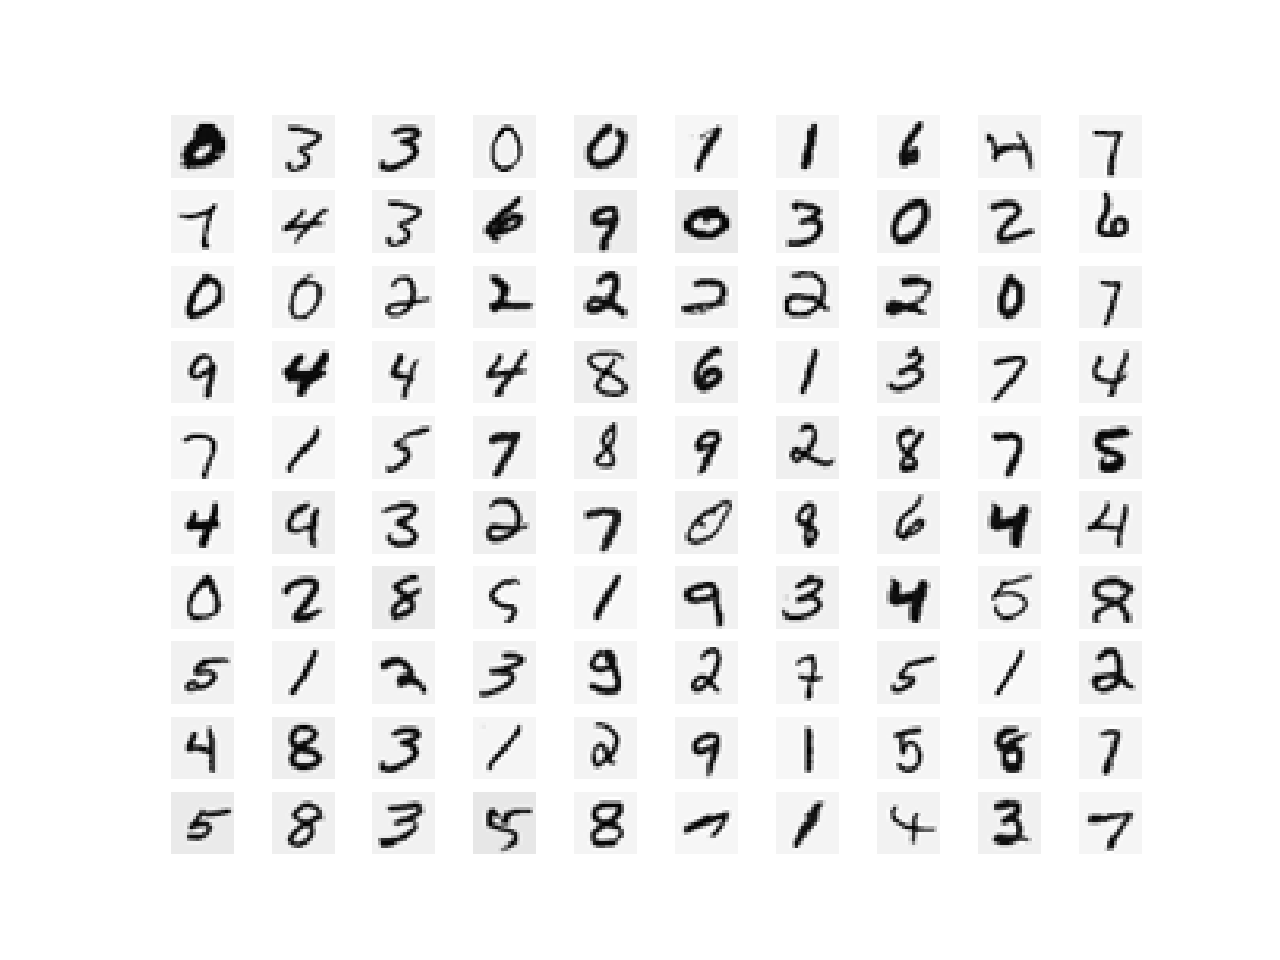
\includegraphics[width=0.6\linewidth]{figs/Chap_6_Figure_0.png}
\end{figure}


\subsection{多分类}

这里采用“一对多”策略完成多分类。对于每一个数字，都单独训练一个逻辑回归分类器：属于当前数字的样本标记为正类，其余数字全部标记为负类。这样便可将一个十分类问题转化为 $10$ 个二分类问题。预测时，分别计算所有分类器给出的概率，并选择概率最大的类别作为最终结果。

沿用上一节的矩阵化正则逻辑回归代码，分别训练 $10$ 个分类器。注意需要在 $X$ 的每一行前添加一个 $1$ 作为偏置项。

\begin{lstlisting}[language=Python]
import numpy as np
from scipy.io import loadmat
import matplotlib.pyplot as plt
import matplotlib

lamb = 1
alpha = 0.1
iteration = 10000
m = 5000
n = 401

data = loadmat('ex3data1.mat')
X = data['X']
X = np.transpose(X.reshape((m, 20, 20)), [0, 2, 1]).reshape(m, 400)
X = np.hstack((np.ones((m, 1)), X))
y = data['y']
y[y==10] = 0

def h(Theta, x):
	return 1 / (1 + np.exp(-np.matmul(Theta.T, x)[0][0]))

def h_(Theta, X):
	return 1 / (1 + np.exp(-np.matmul(X, Theta)))

def J_reg(Theta, X, y):
	tmp = h_(Theta, X)
	return (-(np.matmul(y.T, np.log(tmp)) + np.matmul(1 - y.T, np.log(1 - tmp))) / m\
		 + lamb / 2 / m * np.matmul(Theta.T, Theta))[0][0]

def partJ_reg(Theta, X, y):
	return (np.matmul(X.T, h_(Theta, X) - y) + lamb * np.vstack((np.zeros((1, 1)), Theta[1:, :]))) / m

def GradientDescent(X, y):
	Theta = np.zeros((n, 1))
	for t in range(iteration):
		Theta = Theta - alpha * partJ_reg(Theta, X, y)
	return Theta

def classify(k):
	y_ = y.copy()
	y_[y==k] = 1
	y_[y!=k] = 0
	Theta = GradientDescent(X, y_)
	return Theta

Theta = np.zeros((10, n))
for k in range(10):
	Theta[k, :] = classify(k).flatten()
	print("Trained for:", k)

np.savetxt('theta.txt', Theta, delimiter=',')
\end{lstlisting}

训练得到的参数保存至 \texttt{theta.txt}. 预测时读入该矩阵，对同一个输入同时计算 $10$ 个分类器的输出，再取最大值对应的数字：

\begin{lstlisting}[language=Python]
def predict(Theta, x):
	return np.matmul(Theta, x).argmax(axis=0)
\end{lstlisting}

训练集上各数字的准确率如下。注意：训练集准确率并不能作为模型评估结果，详见第 \ref{sec:chapter9} 章。

\begin{table}[H]
    \centering
    \small
    \begin{tabularx}{\linewidth}{lYYYYYYYYYYY}
    \toprule
    数字 & 0 & 1 & 2 & 3 & 4 & 5 & 6 & 7 & 8 & 9 & Total \\
    \midrule
    准确率 & 99.0\% & 97.8\% & 88.2\% & 90.0\% & 93.4\% & 89.4\% & 97.0\% & 93.8\% & 91.4\% & 91.2\% & 93.1\% \\
    \bottomrule
    \end{tabularx}
\end{table}
